%%
%% Automatically generated file from DocOnce source
%% (https://github.com/hplgit/doconce/)
%%
%%


%-------------------- begin preamble ----------------------

\documentclass[%
oneside,                 % oneside: electronic viewing, twoside: printing
final,                   % draft: marks overfull hboxes, figures with paths
10pt]{article}

\listfiles               %  print all files needed to compile this document

\usepackage{relsize,makeidx,color,setspace,amsmath,amsfonts,amssymb}
\usepackage[table]{xcolor}
\usepackage{bm,ltablex,microtype}

\usepackage[pdftex]{graphicx}

\usepackage{fancyvrb} % packages needed for verbatim environments

\usepackage[T1]{fontenc}
%\usepackage[latin1]{inputenc}
\usepackage{ucs}
\usepackage[utf8x]{inputenc}

\usepackage{lmodern}         % Latin Modern fonts derived from Computer Modern

% Hyperlinks in PDF:
\definecolor{linkcolor}{rgb}{0,0,0.4}
\usepackage{hyperref}
\hypersetup{
    breaklinks=true,
    colorlinks=true,
    linkcolor=linkcolor,
    urlcolor=linkcolor,
    citecolor=black,
    filecolor=black,
    %filecolor=blue,
    pdfmenubar=true,
    pdftoolbar=true,
    bookmarksdepth=3   % Uncomment (and tweak) for PDF bookmarks with more levels than the TOC
    }
%\hyperbaseurl{}   % hyperlinks are relative to this root

\setcounter{tocdepth}{2}  % levels in table of contents

% --- fancyhdr package for fancy headers ---
\usepackage{fancyhdr}
\fancyhf{} % sets both header and footer to nothing
\renewcommand{\headrulewidth}{0pt}
\fancyfoot[LE,RO]{\thepage}
% Ensure copyright on titlepage (article style) and chapter pages (book style)


\pagestyle{fancy}


% prevent orhpans and widows
\clubpenalty = 10000
\widowpenalty = 10000

% --- end of standard preamble for documents ---


% insert custom LaTeX commands...

\raggedbottom
\makeindex
\usepackage[totoc]{idxlayout}   % for index in the toc
\usepackage[nottoc]{tocbibind}  % for references/bibliography in the toc

%-------------------- end preamble ----------------------

\begin{document}

% matching end for #ifdef PREAMBLE

\newcommand{\exercisesection}[1]{\subsection*{#1}}


% ------------------- main content ----------------------



% ----------------- title -------------------------

\thispagestyle{empty}

\begin{center}
{\LARGE\bf
\begin{spacing}{1.25}
Project 4, Phase Transitions in the Two Dimensional Ising Model
\end{spacing}
}
\end{center}

% ----------------- author(s) -------------------------

\begin{center}
{\bf \href{{https://github.com/mathhat/prosjekt4}}{Link to Git / Code}}
\end{center}

% ----------------- end author(s) -------------------------

% --- begin date ---
\begin{center}
Fall 2016
\end{center}
% --- end date ---

\vspace{1cm}

\begin{abstract}
 In this project I've implemented and parallelized the metropolis algorithm using C++ and Open MPI in order to create an efficient Ising model.
 We've found analytical expressions for attributes such as spin and energy in order to compare them with our numerical results. The comparison with numerical results did not go
 well for anything else than magnetism. We've looked at the different attributes behaviour for longer cycles and varying temperatures in order to find linear relations between
 accepted states cycles and temperatures. From the data we created probability distributions and graphs of accepted states. After finding the most 
 probable states, we looked at how all attributes behaved as we increased the temperature to to $T_C$. Sadly, my algorithm exposed to phase transition.
\end{abstract}

\subsection*{Studies of phase transitions in magnetic systems}

\section*{Introduction}
This project focuses on the popular Ising model to simulate phase transitions in two dimensions. The system this model creates has a critical temperature where a 
phase transition takes place. The transition from a magnetic phase (a system with a finite magnetic moment) to a phase with zero magnetization. What we mean by magnetization is the number of spins aligned in the same direction.
In other words, we're going to heat up a magnet and expect its field to disappear.
\\
\\
We're going to look at not only magnetization $\langle|M|\rangle$, but also changes is energy $\langle E\rangle$, equilibrium states, heat capacity/specific heat $\langle C_V\rangle$ and susceptibility $\langle \chi \rangle$ as functions of time or temperature.

The energy of the Ising model can be expressed as,
\[
E=-J\sum_{< kl >}^{N}s_ks_l 
\]
without an externally applied magnetic field, 
with
$s_k=\pm 1$. $N$ represents number of spins, $J$ is a coupling
constant expressing the significance of the interaction between
neighboring spins and $<kl>$ indicates that we sum over
nearest neighbors only. For ferromagnetic structures, $J> 0$.  We will use periodic boundary conditions and
the Metropolis algorithm. 

\section*{2 by 2 Example}

To kick off, we have 4 spins. An $L\times L$ matrix where $L=2$. We want to express the magnetization, energy, specific heat and susceptibility.
\subsection*{Energy}
To express the energy of this model, we can simply find the derivative of its states, $Z$.
\begin{equation}
 \label{Z}
 Z = \sum_{j}^{N_e} g(j)e^{-\beta E_{i,j}}
\end{equation}

Z is called the partition function and has a valuable relation to energy and its degeneration.
The sum in equation \ref{Z} goes up to $N_e$ which refers to the number of unique energy states.
Since we have degeneration, where multiple states possess the same energy, we need the coefficient $g(j)$ which equals the number of states possessing the energy $E_{j}$.
\begin{table}
\begin{center}
\begin{tabular}{|c  c  c  c | }
  \hline
   Number spins up    &Degeneracy& Energy & Magnetization \\ \hline
   4 & 1 & -8J&4  \\ \hline
   3 & 4 & 0&  2 \\ \hline
   2 & 4 & 0&  0\\ \hline
   2 & 2 & 8J& 0 \\ \hline
   1 & 4 & 0&  -2\\ \hline
   0 & 1 & -8J& -4 \\ 
  \hline
\end{tabular}
\caption{Table shows the states' energy, degeneracy and magnetization for $L=2$ }
\label{tab1}
\end{center}
\end{table}
We see that we only have three possible energies in table \ref{tab1}
Which means that the partition function can be written with tree terms, one for each energy:
\begin{equation}
\begin{split}
  Z =& \sum_{j}^{N_e} g(j)e^{-\beta E_{i,j}} \\
  \implies Z =& 2e^{\beta 8J} + 12 + 2e^{-8\beta J}
\end{split}
 \end{equation}
With the partition for $L=2$, we can find the energy with the relation
$$\langle E \rangle = -\frac{1}{Z} \frac{d\langle E \rangle}{d\beta}$$
Finding the derivative we get
\begin{equation}
\begin{split}
  \langle E \rangle =& -\frac{1}{Z} \frac{d\langle E \rangle}{d\beta} \\
  \implies \langle E \rangle =& -8J\frac{e^{\beta 8J} - e^{-8\beta J}}{e^{\beta 8J} + 6 + e^{-8\beta J}}
\end{split}
 \end{equation}
\subsection*{Specific Heat}
Now that we possess the energy, let's get the specific heat out of the way:
$$C_V = \frac{d \langle E \rangle}{dT} = -\frac{1}{kT^2} \frac{d \langle E \rangle}{d\beta}$$
Inserting the energy into the expression we get
\begin{equation}
\begin{split}
 \langle C_V \rangle =& \frac{d\langle E \rangle}{dT} = kT^2 \frac{d\langle E \rangle}{d\beta} \\
\implies C_V =& 8JkT^2 \frac{d}{d\beta}\frac{e^{\beta 8J} - e^{-8\beta J}}{e^{\beta 8J} + 6 + e^{-8\beta J}}\\
=& \\
 =& (8J)^2kT^2\left( \frac{(e^{\beta 8J} + e^{-8\beta J})}{e^{\beta 8J} + 6 + e^{-8\beta J}} - \frac{(e^{\beta 8J} - e^{-8\beta J})^2}{(e^{\beta 8J} + 6 + e^{-8\beta J})^2} \right)\\
 & \\ 
 =& (8J)^2kT^2\left(\frac{\cosh{(8\beta J)}}{\cosh{(8\beta J)} + 3 } - \frac{\sinh{(8\beta J)}}{(\cosh{(8\beta J)} + 3)^2} \right)\\
 & \\ 
 =& (8J)^2kT^2\left(\frac{3\cosh{(8\beta J) + 1}}{(\cosh{(8\beta J)} + 3)^2} \right)
 \end{split}
 \end{equation}
\subsection*{Magnetization}
 The magnetization is simply the sum of spins. Since we don't discriminate between the up and down direction (after the sum has been counted), we choose to look at the absolute value:
\begin{equation}
 \label{M}
 \langle |M| \rangle =\left|\sum_{i}^{L}\sum_{j}^{L} s_{i,j}\right|
\end{equation}
the spins, $s_{i,j} =$ ±1, therefore magnetization can range from and to $±L^2$.
The analytical expectation value is expresses as
\begin{equation}
\begin{split}
\langle |M| \rangle =& \frac{1}{Z} \sum_j^{N_e} |M_j| e^{-\beta E_j} \\
=& \frac{8e^{8J\beta} + 4}{2e^{\beta 8J} + 12 + 2e^{-8\beta J}} \\
&\\
=& \frac{16e^{8J\beta} + 8}{4\cosh{(8\beta J)} +  12 }
\end{split}
\end{equation}

\subsection*{Susceptibility}
The magnetic susceptibility is expressed as the variance of magnetization over $kT$:
\begin{equation}
\begin{split}
\langle  \chi  \rangle =& \frac{\sigma_M^2}{kT}\\
 =& \langle |M^2| \rangle - (\langle |M| \rangle)^2 \\
 =& \left( \frac{32e^{8J\beta} + 16}{4\cosh{(8\beta J)} +  12 }\right) - \left(\frac{16e^{8J\beta} + 8}{4\cosh{(8\beta J)} +  12 }\right)^2
\end{split}         
\end{equation}
Let's just leave susceptibility at that..


\section{Simulation of 2 by 2 system}
After writing a code that creates a probability barrier for phase transitions, called the Metropolis algorithm (basically a smart randomwalker),
we start analysing the attributes expressed earlier.
\subsection{Susceptibility and Specific Heat}
No mather how many Monte Carlo Cycles the Metropolis algorithm runs, my results are quite rotten.
I will however show you the result as a function of time.

The exact $C_V$ equals $0.12$, while my code prefers the number $0.16$, and don't get me started on susceptibility.
The energy and magnetism behaves, luckily, better.
\subsection{Energy and Magnetism}
\begin{table}
\begin{center}
\begin{tabular}{|c  c  c | }
  \hline
   MC Cycles ($10^x$)   &Energy & Magnetization \\ \hline
   3 & -2.3735015J & 0.97215285  \\ \hline
   4 & -2.3593516J & 0.98661384 \\ \hline
   5 & -2.3593516J & 0.98902136\\ \hline
   6 & -2.3587971J & 0.98387202 \\ \hline
   7 & -2.3587898J & 0.98177351\\ 
  \hline
\end{tabular}
\caption{Table shows the energy and magnetization for $L=2$ for different amounts of cycles. Energy should be approximately 2, Magnetization 1}
\label{tab1}
\end{center}
\end{table}
So these are ok results for magnetization, but not too good energy values.The fact that the magnetization is accurate makes me think that I at some point mess with the energy, but the algorithm as a whole
still works.
\section{Equilibrium}
The amount og cycles interated through can here be thought of as time.
Over a great amount of cycles, our model goes towards something looking like an equilibrium state.
We're going to vary our time/MC cycles in order to pinpoint exactly where this happens.
Using a $20\times20$ matrix, the following plots (\ref{1} and \ref{2}) are created by slowly increasing the cycles while measuring energy and magnetization:
\begin{figure}
 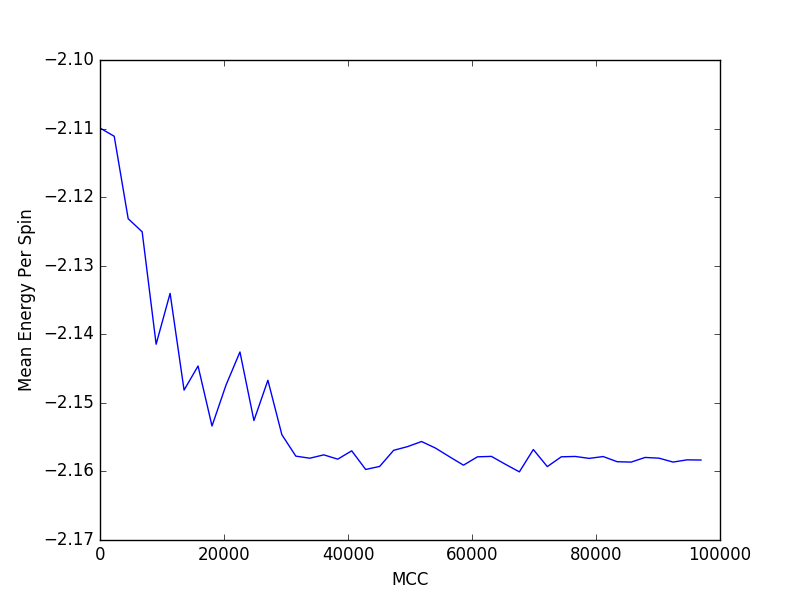
\includegraphics[scale=0.5]{1}
 \caption{Energy States reaches equilibrium over time, around MCC = 30k}
 \label{1}
 \end{figure}
\begin{figure}
 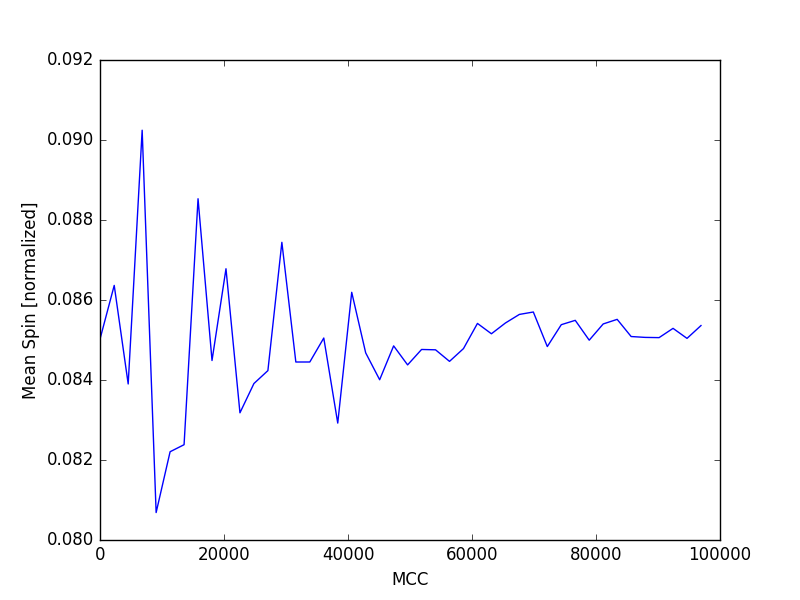
\includegraphics[scale=0.5]{2}
 \caption{Mean Magnetization reaching equilibrium a while later than energy.}
 \label{2}
\end{figure}
We can clearly observe that the system goes towards a near equilibrium condition.
\section{Acceptance}
The Metropolis algorithm we're using has a probability barrier when it comes to accepting states of higher than previous energies.
To find see how the number of accepted states behave as a function of time and temperature, I've gathered some data from an 
$L = 10$ simulation. I plot \ref{accept} and \ref{acceptt}, you'll  find the number of accepted states as a function of monte carlo cycles (at T = 1) and
of a varying temperature. 
\begin{figure}
 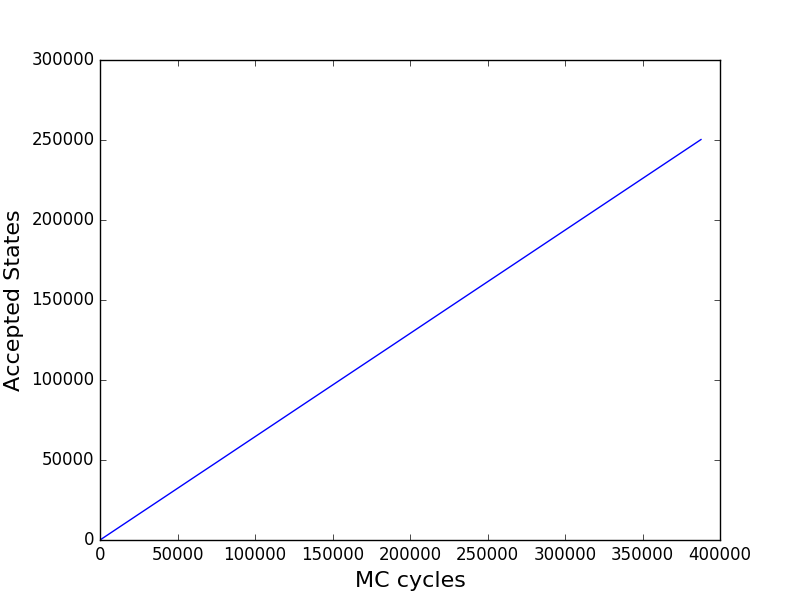
\includegraphics[scale=0.5]{accept}
 \caption{The growth is linear when the number of cycles vary from max MCC = 40 to MCC = 80 000. Time will not change the growth rate of accepted state behavoiour}
 \label{accept}
 \end{figure}
\begin{figure}
 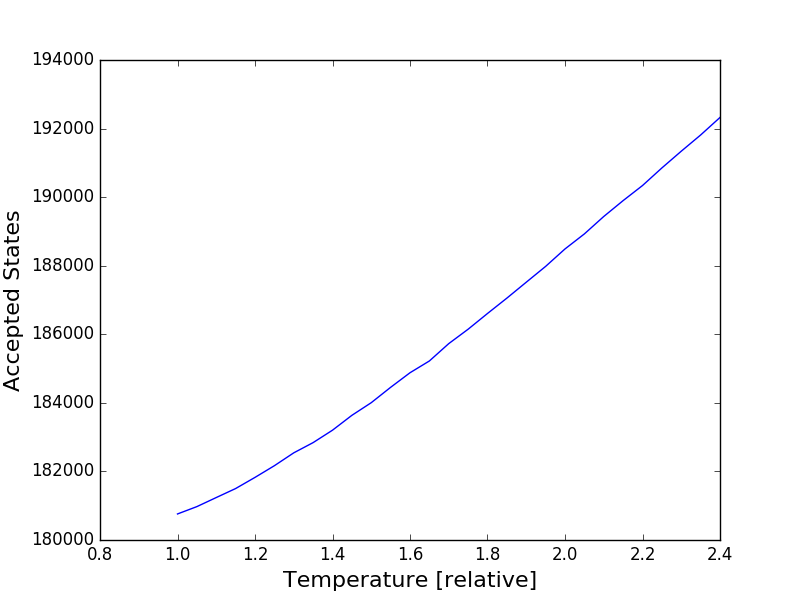
\includegraphics[scale=0.5]{acceptt}
 \caption{When temperature is risen from 1 to 2.4, we observe an interesting curve, but as the temperature's grow higher, linear growth appears.}
 \label{acceptt}
\end{figure}

\subsection{PDF}
To map the equilibrium state and other probable states, we can use histogram algorithms and the spline interpolation method.
Since numpy/scipy of Python are our friends, we will use their versions: scipy.interpolate.UnivariateSpline and numpy.histogram.
For lower temperatures, we observe that lower energy states are inhabited. We also observe a different shape of their distribution.
Low temperatures lean to the left as we see in figure \ref{low} and opposite for the higher ones \ref{high}. The variance of the energy was too big to fit these distributions. 
\begin{figure}
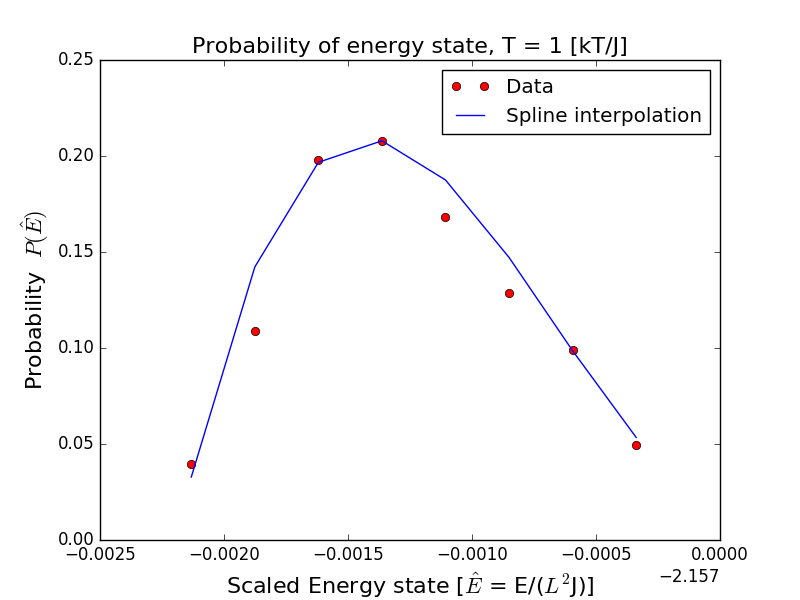
\includegraphics[scale=0.5]{bestfitt1}
\caption{The probability distribution of the Ising model for low temperatures T=1. It's tilting strongly to the left.}
\label{low}
\end{figure}
\begin{figure}
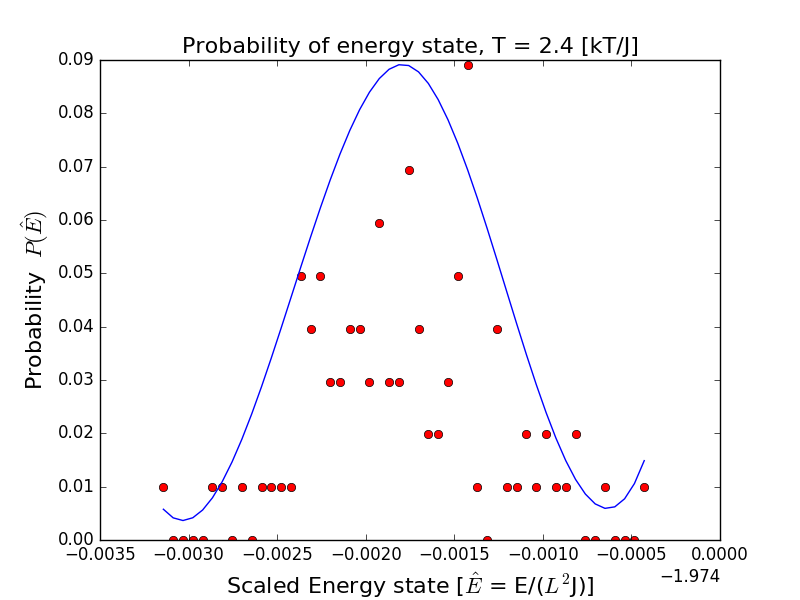
\includegraphics[scale=0.5]{bestfitt2} 
\caption{The most probable states for T=2.4, these are for higher energies and the distribution's shape is now tilting weakly to the right.}
\label{high}
\end{figure}


\section{Heating to Phase Transition}
We wish to study the behavior of the Ising model
in two dimensions close to the critical temperature as a function of
the lattice size $L\times L$. To do this, we calculate the expectation values for
$\langle E\rangle$ and $\langle \vert M\vert \rangle$, the specific heat
$C_V$ and the susceptibility $\chi$ as functions of $T$ and $L$.
\\
\\
When $L$ becomes higher, the number of flops grow exponentially $\sim$ $L^2$.
This means when $L$ is as high as 100, my cycles have been reduced to 15k,
while for $L=2$, the cycles can be so many as $maxMCC = 10^7$.

\begin{figure}
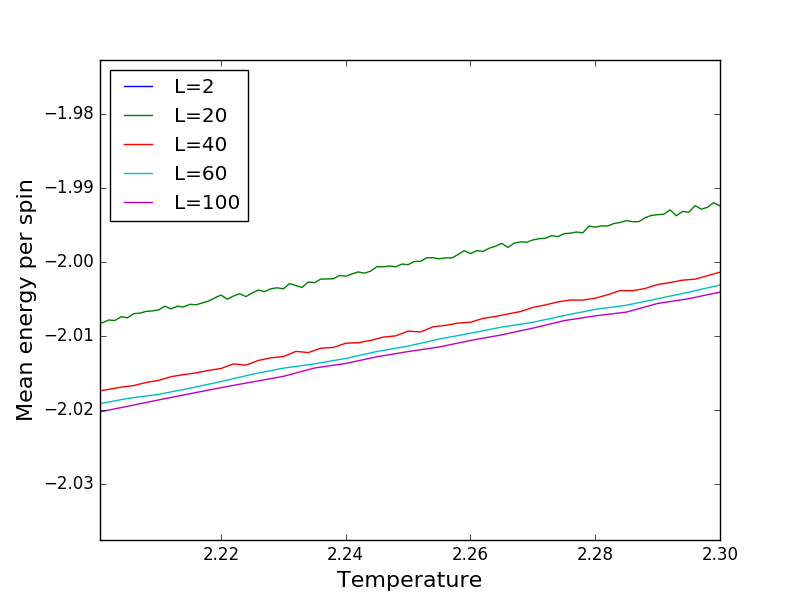
\includegraphics[scale=0.5]{energy}
\caption{The rises linearly for all systems. No transition observed.}
\label{low}
\end{figure}
\begin{figure}
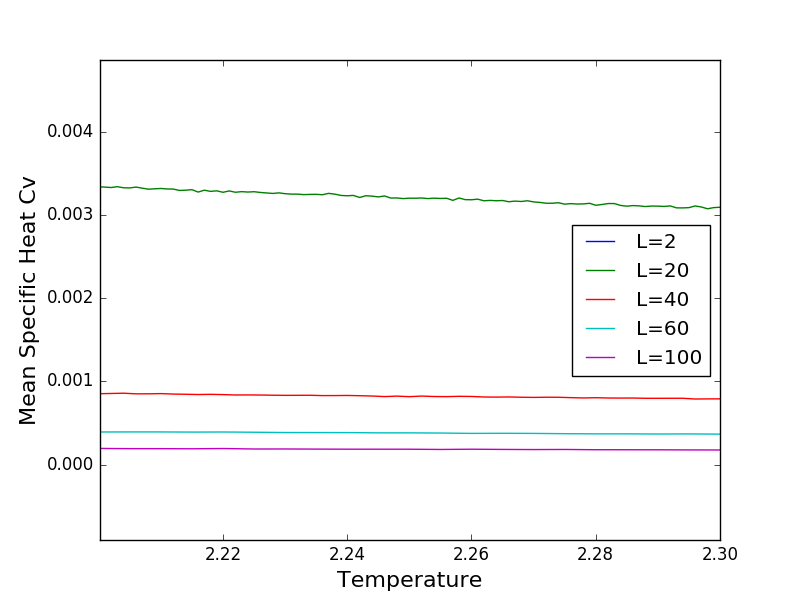
\includegraphics[scale=0.5]{cv'} 
\caption{Specific is low and barely diminishing.}
\label{high}
\end{figure}

\begin{figure}
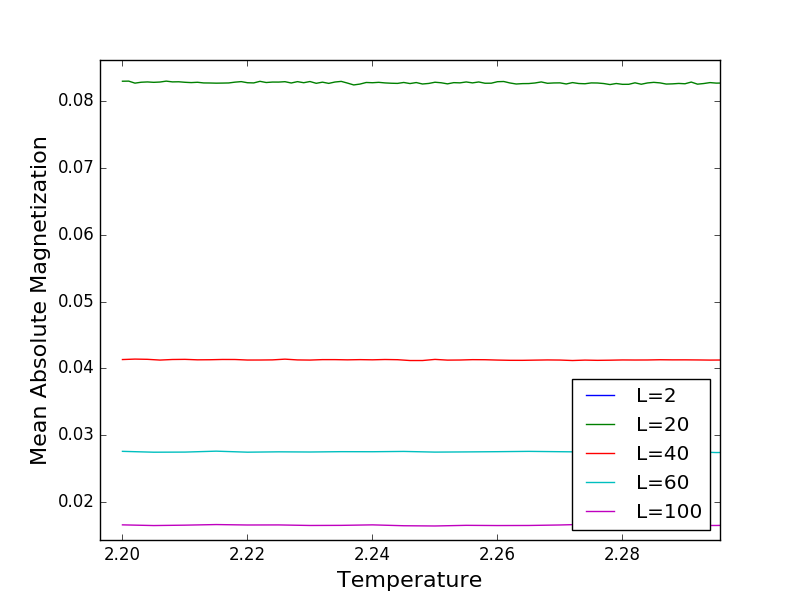
\includegraphics[scale=0.5]{mag}
\caption{Magnetism is constantly in equilibrium}
\label{low}
\end{figure}
\begin{figure}
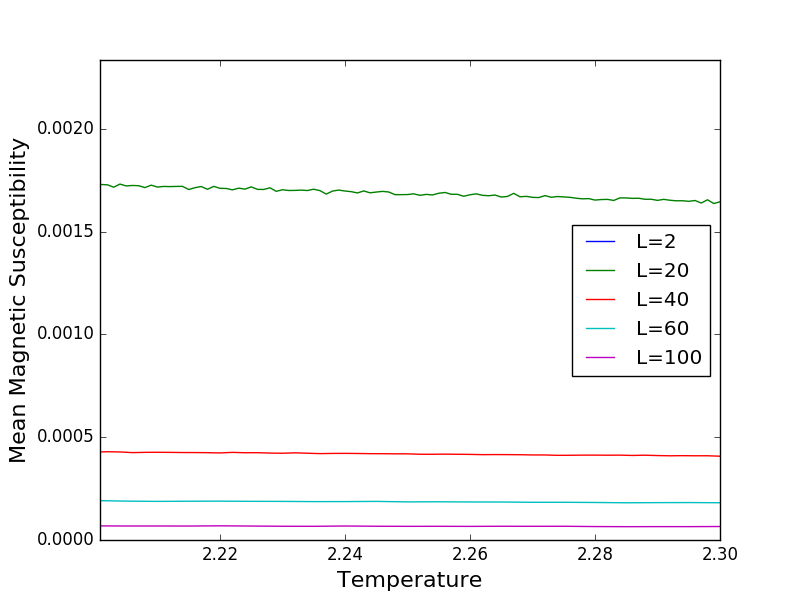
\includegraphics[scale=0.5]{susceptibility} 
\caption{Susceptibility is almost identical to Specific Heat and shows no sign transitions.}
\label{high}
\end{figure}

\section{Critical Temperature}
The phase transition happens around the critical/Curie temperature.
This was not observed in my simulations, perhaps due to a lack of sampling, or just incompetent code.

\section{Conclusion}
We have seen how the Ising model can be merged modeled with the metropolis algorithm, and using random Monte Carlo steps, describes a system of spins.
We've observed the behaviour of the system by increasing time/Monte Carlo cycles, and by increasing temperature. Doing this, we've seen that the model is trying to reach an equilibrium state,
it uses a probability distribution, it's amount of accepted states are a linear function of time and temperature and that temperature increase causes rise in energy and phase transitions (Although, 
I was not able to prove the last one myself).








% ------------------- end of main content ---------------

\end{document}

